% Created 2024-01-30 Tue 14:39
% Intended LaTeX compiler: pdflatex
\documentclass[presentation]{beamer}
\usepackage[utf8]{inputenc}
\usepackage[T1]{fontenc}
\usepackage{graphicx}
\usepackage{longtable}
\usepackage{wrapfig}
\usepackage{rotating}
\usepackage[normalem]{ulem}
\usepackage{amsmath}
\usepackage{amssymb}
\usepackage{capt-of}
\usepackage{hyperref}
\mode<beamer>{\usetheme{Madrid}}
\definecolor{SUred}{rgb}{0.59375, 0, 0.17969} % SU red (primary)
\definecolor{SUblue}{rgb}{0, 0.17578, 0.38281} % SU blue (secondary)
\setbeamercolor{palette primary}{bg=SUred,fg=white}
\setbeamercolor{palette secondary}{bg=SUblue,fg=white}
\setbeamercolor{palette tertiary}{bg=SUblue,fg=white}
\setbeamercolor{palette quaternary}{bg=SUblue,fg=white}
\setbeamercolor{structure}{fg=SUblue} % itemize, enumerate, etc
\setbeamercolor{section in toc}{fg=SUblue} % TOC sections
% Override palette coloring with secondary
\setbeamercolor{subsection in head/foot}{bg=SUblue,fg=white}
\setbeamercolor{date in head/foot}{bg=SUblue,fg=white}
\institute[SU]{Shenandoah University}
\titlegraphic{
\includegraphics[width=0.5\textwidth]{\string~/Documents/suLogo/suLogo.pdf}}
\usetheme{default}
\author{Chase Mathison\thanks{cmathiso@su.edu}}
\date{31 January 2024}
\title{Area between curves}
\hypersetup{
 pdfauthor={Chase Mathison},
 pdftitle={Area between curves},
 pdfkeywords={},
 pdfsubject={},
 pdfcreator={Emacs 29.1 (Org mode 9.6.7)}, 
 pdflang={English}}
\begin{document}

\maketitle

\section{Announcements}
\label{sec:org35c771a}
\begin{frame}[label={sec:org51b92f0}]{Announcements}
\begin{enumerate}
\item Stay up to date on homework!
\item Office hours: M - F, 10am - 11am.
\end{enumerate}
\end{frame}

\begin{frame}[label={sec:org8484c41}]{Another way}
Let's look at a different way to do this problem:

Find the area bounded by the curves defined by the functions
\[ f \left( x \right) = x^2, \quad g \left( x \right) = 2-x, \quad h
\left( x \right) = 0. \]
for \(0 \le x \le 2.\)

\begin{center}
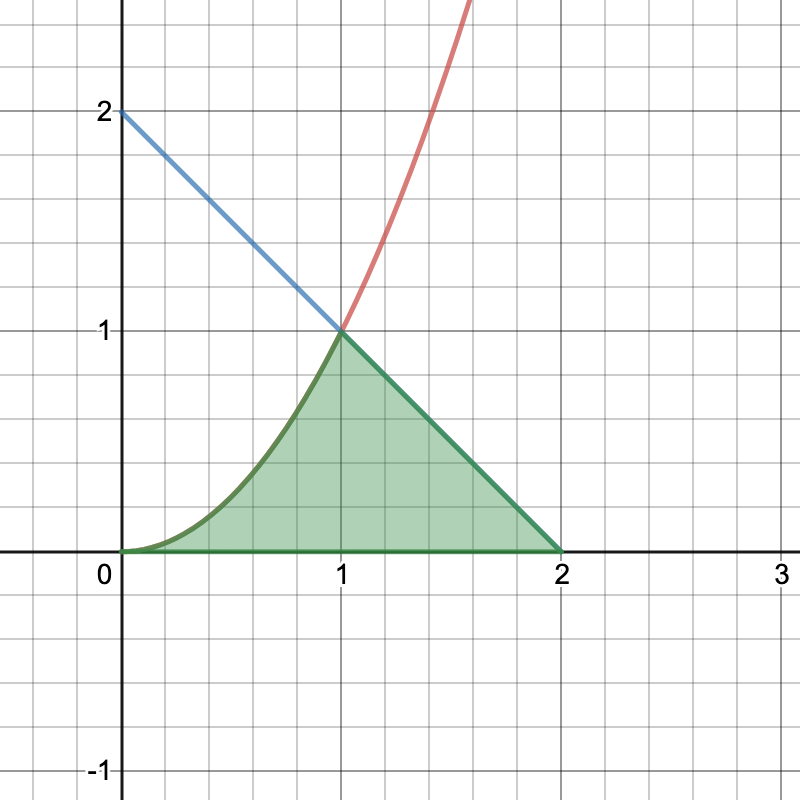
\includegraphics[width=0.4\textwidth]{../img/day005-ex1.png}
\end{center}
\end{frame}

\begin{frame}[label={sec:orge76f691}]{Another way}
To find this area last time, we had to break this area into 2 pieces
and then find the areas separately.

A way to tackle this problem all at once is to instead switch to
integrating in terms of \uline{\hspace*{1in}} instead of in terms of \(x\).

When we do this, instead of a ``top'' curve and a ``bottom'' curve, we are
really looking at a \uline{\hspace*{1in}} curve and a \uline{\hspace*{1in}} curve.

Let's try to tackle this area by integrating in terms of \(y\)
instead of \(x\).
\end{frame}

\begin{frame}[label={sec:org42e986c}]{Example}
Find the area bounded by the curves defined by the functions
\[ f \left( x \right) = x^2, \quad g \left( x \right) = 2-x, \quad h
\left( x \right) = 0. \]
for \(0 \le x \le 2,\) by integrating with respect to the dependent
variable instead of the independent variable.
\vspace{10in}
\end{frame}

\begin{frame}[label={sec:orgb871cfa}]{Example}
\end{frame}

\begin{frame}[label={sec:org0995c76}]{How it works in general}
In general, if we want to find the area bounded by two functions of
\(y\), we can use the ``little slice'' method as follows:
\vspace{10in}
\end{frame}

\begin{frame}[label={sec:org71b9298}]{How it works in general}
\end{frame}

\begin{frame}[label={sec:org9d0d93f}]{Example}
Find the area of the region bounded by the curves
\[ y = \frac{1}{x^2}, \, y = 2x, \, y = 2. \]
\begin{center}
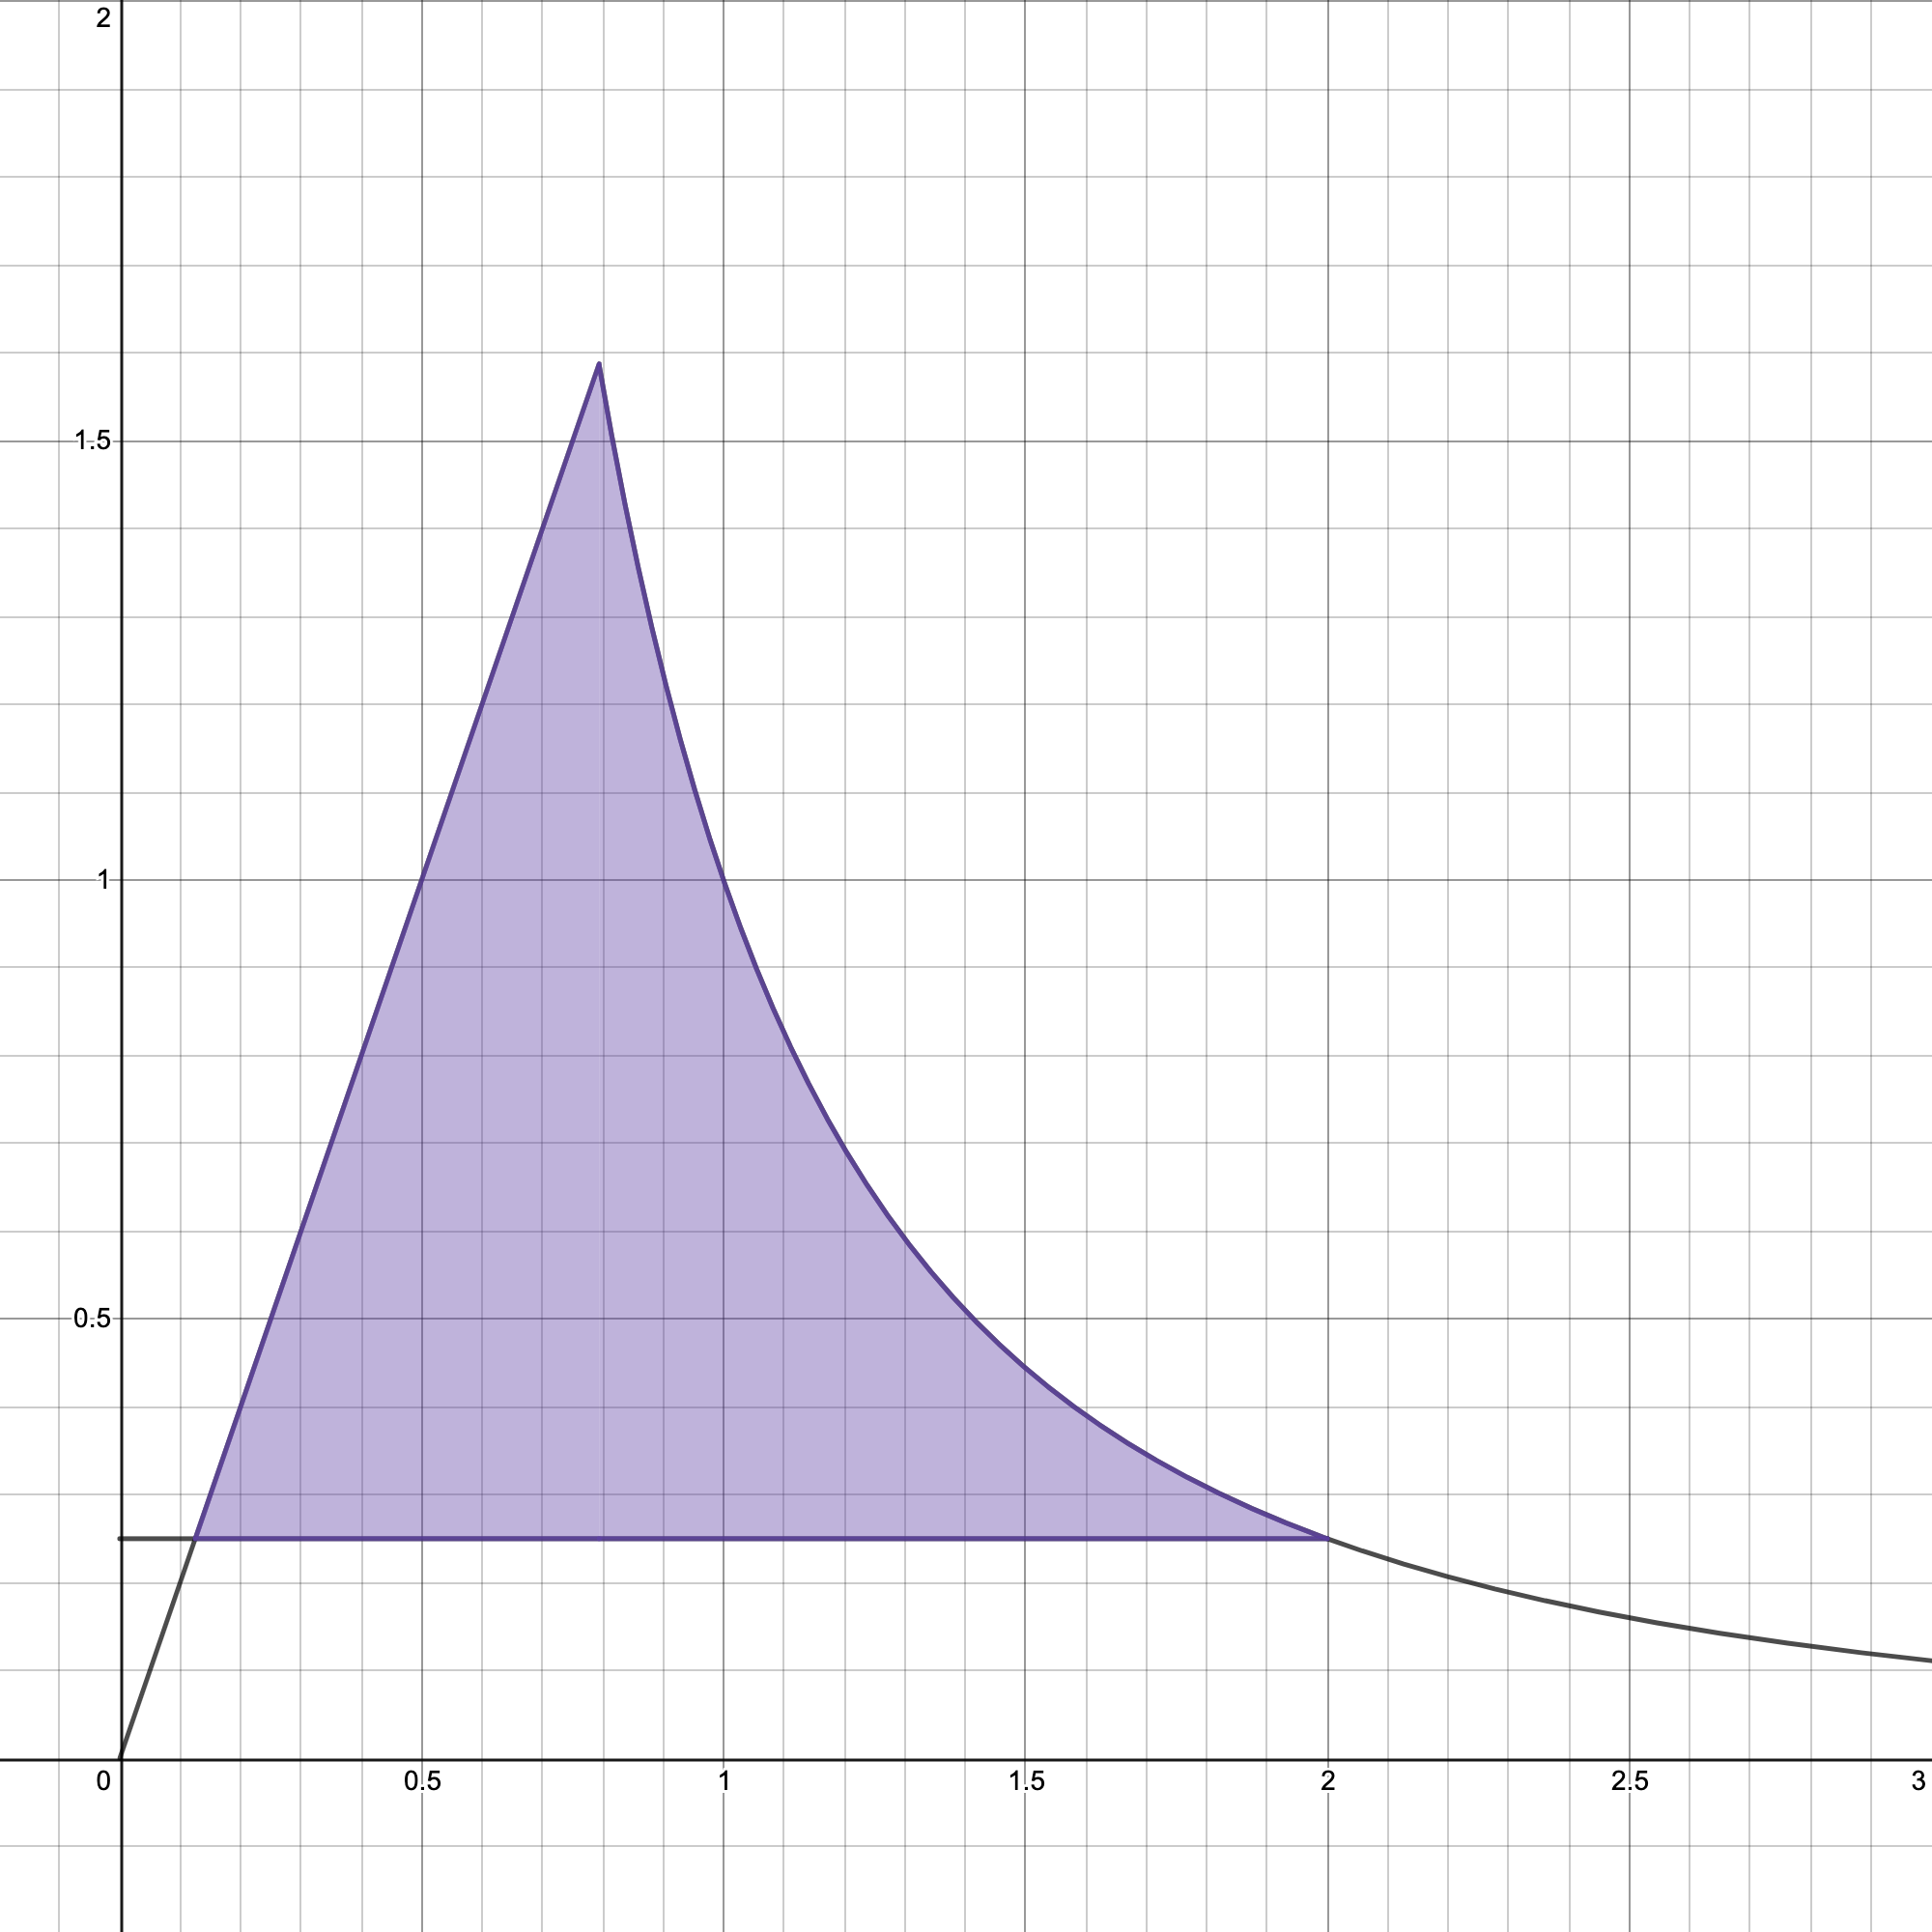
\includegraphics[width=0.5\textwidth]{../img/day005-ex2.png}
\end{center}
\end{frame}

\begin{frame}[label={sec:orga091098}]{Example}
\end{frame}
\end{document}